\documentclass[12pt]{article}
\usepackage{amsmath, amssymb, amsthm, commath, enumitem, graphicx, nopageno, quoting}
\usepackage[margin=1cm]{geometry}

\title{Computer Science 452 - Homework Assignment \#4}
\author{Hari Amoor, NetID: hra25}
\date{February 18, 2020}

\begin{document}
\maketitle
\section*{Problem 2.4e: Generate a CFG for the language of palindromes.}
The CFG required is as follows, for $\alpha \in \Sigma$:
\begin{align*}
  A \rightarrow \epsilon \\
  A \rightarrow \alpha \\
  S \rightarrow \alpha S \alpha
\end{align*}

\section*{Problem 2.5: Give informal descriptions and state diagrams of PDAs for Problem 2.4e.}
The PDA $M$ that recognizes the language of bit-wise palindromes is as follows: \\
\newline
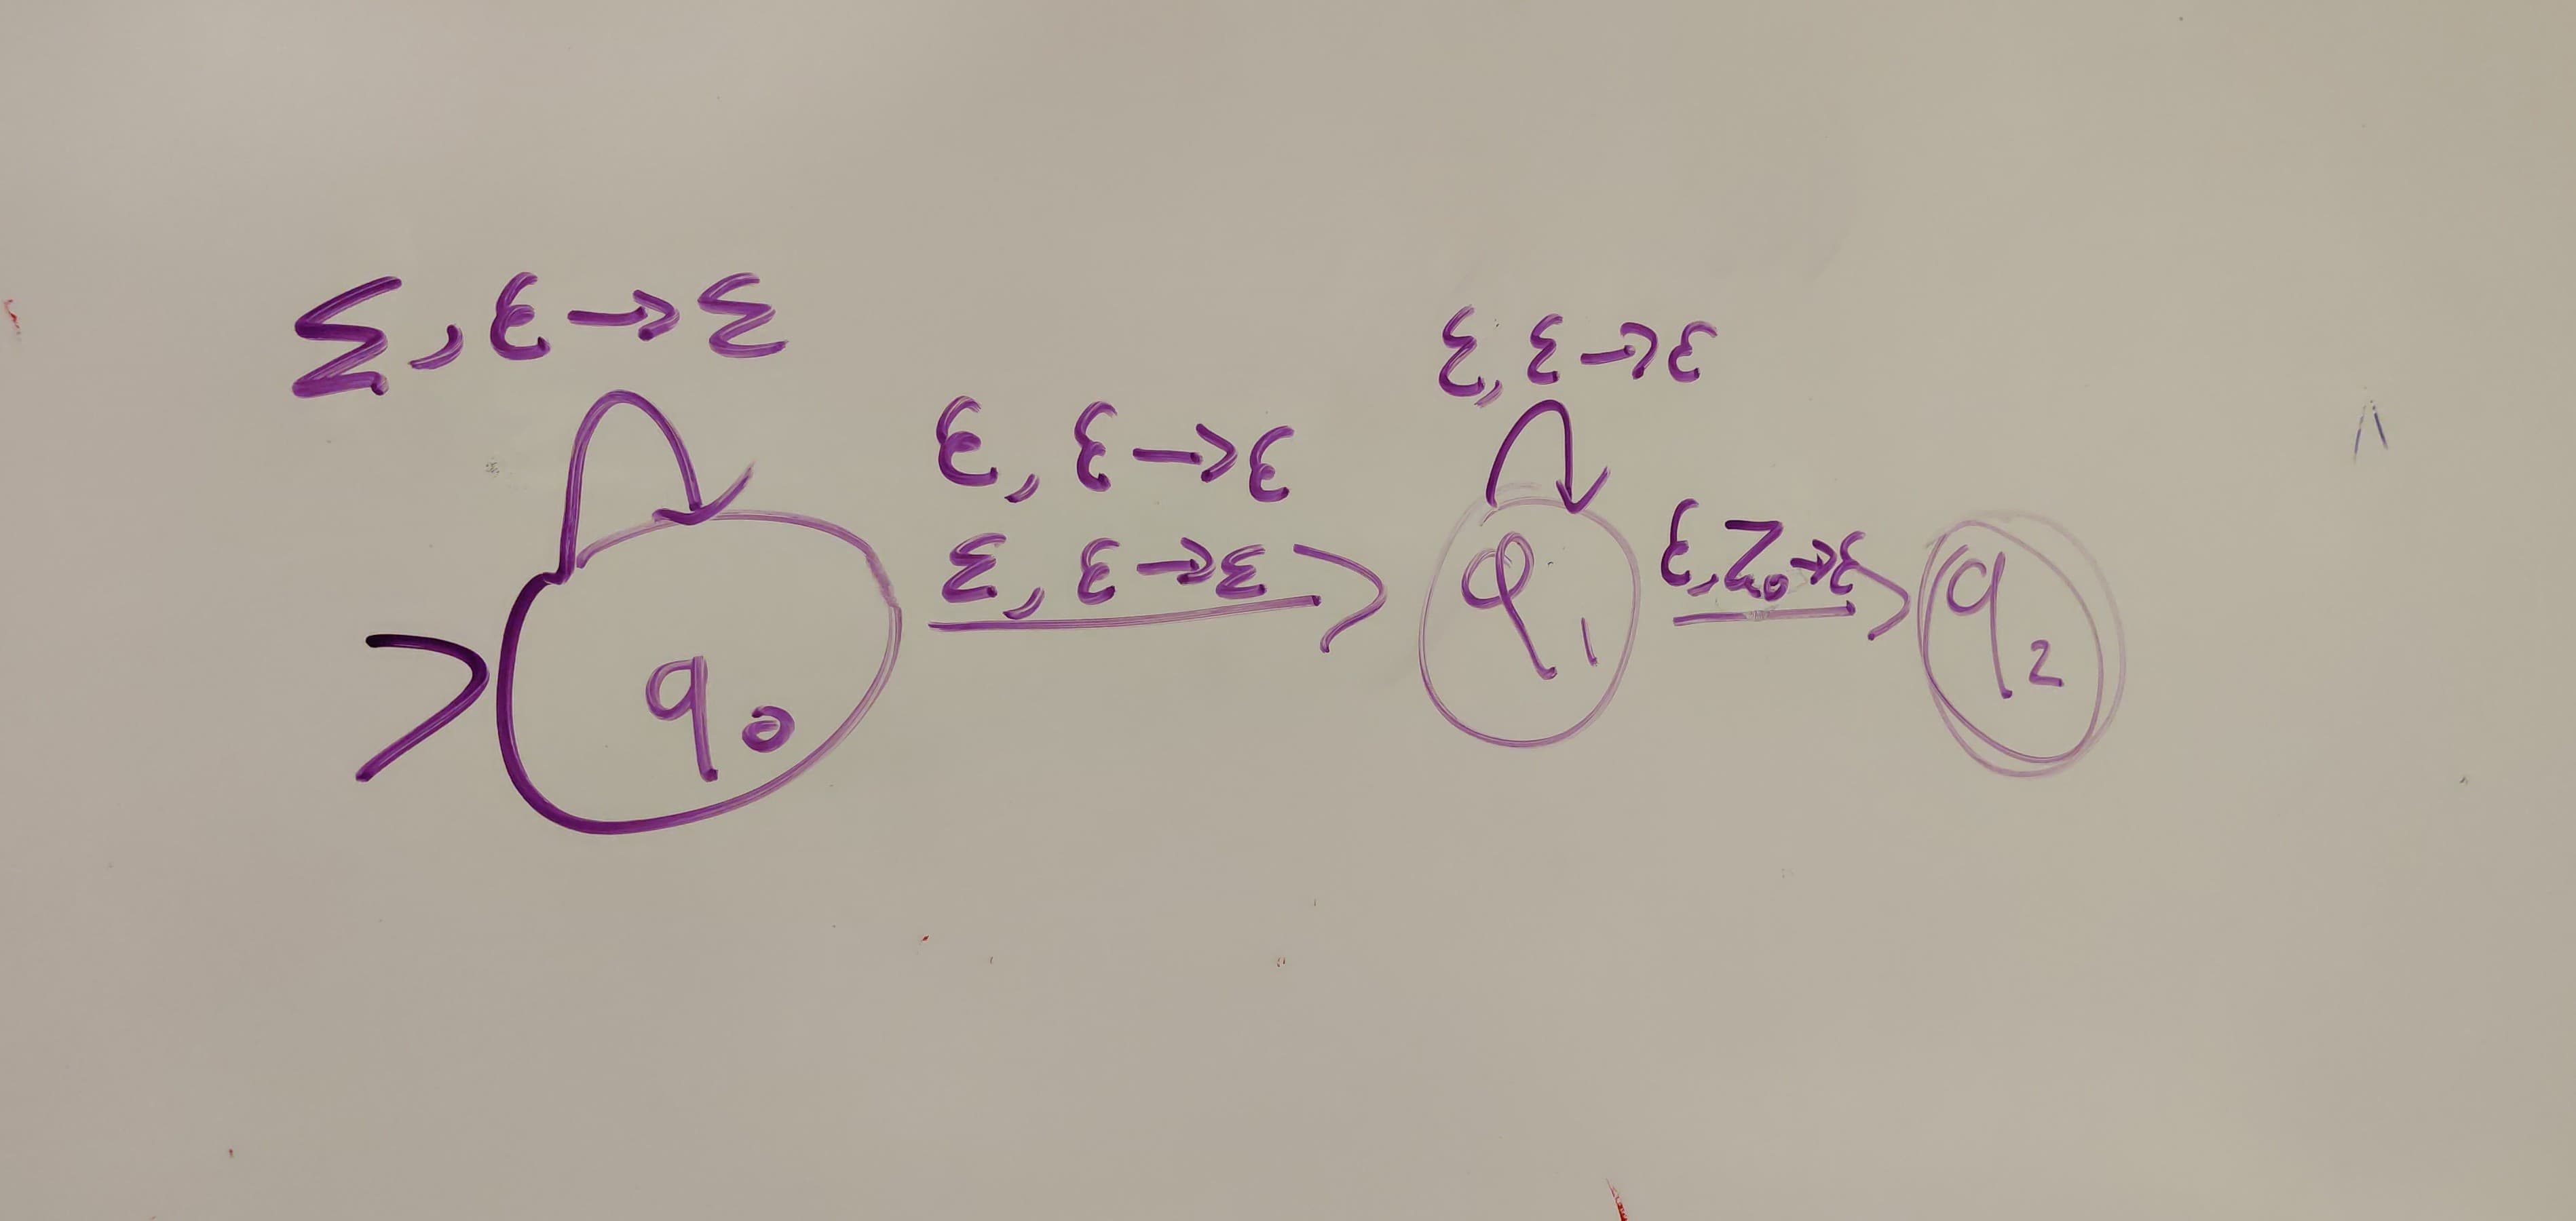
\includegraphics[width=\linewidth]{images/problem25.jpg}

\section*{Problem 2.9: Provide a CFG that computes $A = \{a^{i}b^{j}c^{k} \mid i = j \text{ or } j = k\}$.}
The CFG to compute the superset $A_{1}$ of the language where $i = j$ is as follows:
\begin{align*}
  S_{1} \rightarrow aS_{2}bS_{3} \mid \epsilon \\
  S_{2} \rightarrow aS_{2}b \mid \epsilon \\
  S_{3} \rightarrow cS_{3} \mid \epsilon
\end{align*}
The CFG to compute the superset $A_{2}$ of the language where $j = k$ is as follows:
\begin{align*}
  S_{4} \rightarrow S_{5}bS_{6}c \mid \epsilon \\
  S_{5} \rightarrow cS_{5} \mid \epsilon \\
  S_{6} \rightarrow bS_{6}c \mid \epsilon
\end{align*}
$A$ is the language given by the grammar:
\begin{align*}
  S_{0} \rightarrow S_{1} \mid S_{4}
\end{align*}

\section*{Problem 2.10: Informally describe a PDA of the language described in Problem 2.9.}
The PDAs to describe the languages $A_{1}$ and $A_{2}$ are trivial. We observe that $A = A_{1} \cup A_{2}$, and extending PDAs with union over their languages is also trivial.

\section*{Problem 2.14: Convert the given CFG to Chomsky-Normal Form.}
The equivalent description of the CFG is as follows:
\begin{align*}
  S \rightarrow BC \mid AB \mid BA \mid ZZ \mid \epsilon \\
  A \rightarrow BC \mid AB \mid BA \mid ZZ \\
  B \rightarrow ZZ \\
  C \rightarrow AB \\
  Z \rightarrow 0
\end{align*}

\section*{Problem 2.35, Claim: Let $G$ be a CFG that contains at least $b$ variables. Then, if $G$ generates some string with a derivation of at least $2^{b}$ steps, then $L(G)$ is infinite.}
\begin{proof}
  W.l.o.g., assume $G$ is in Chomsky-Normal Form. Then, every derivation can generate at most two terminal symbols, so the parse tree using $G$ must have height at most $2^{b} - 1$. \\
  \newline
  Trivially, it must be the case that the parse tree has height at least $b + 1$. Thus, there is a path from root to leaf of length $b + 1$. By the Pigeonhole Principle, at least one variable $A$ occurs twice. \\
  \newline
  This is sufficient to show that the CFL generated by $G$ is infinite.
\end{proof}


\end{document}